\documentclass[tikz,border=10pt]{standalone}
\usepackage[utf8]{inputenc}
\usepackage[T1]{fontenc}
\usepackage{amsmath,amssymb}
\usepackage{tikz}
\usetikzlibrary{shapes.geometric, arrows.meta, positioning, calc, fit, backgrounds}

\definecolor{primary}{HTML}{0F172A}
\definecolor{primaryblue}{HTML}{1E3A8A}
\definecolor{accentblue}{HTML}{0284C7}
\definecolor{tealaccent}{HTML}{0D9488}
\definecolor{darkgreen}{HTML}{065F46}
\definecolor{lightgreen}{HTML}{ECFDF5}
\definecolor{crimson}{HTML}{991B1B}
\definecolor{lightred}{HTML}{FEF2F2}
\definecolor{amber}{HTML}{B45309}
\definecolor{lightamber}{HTML}{FFFBEB}
\definecolor{boxbg}{HTML}{F8FAFC}

\begin{document}

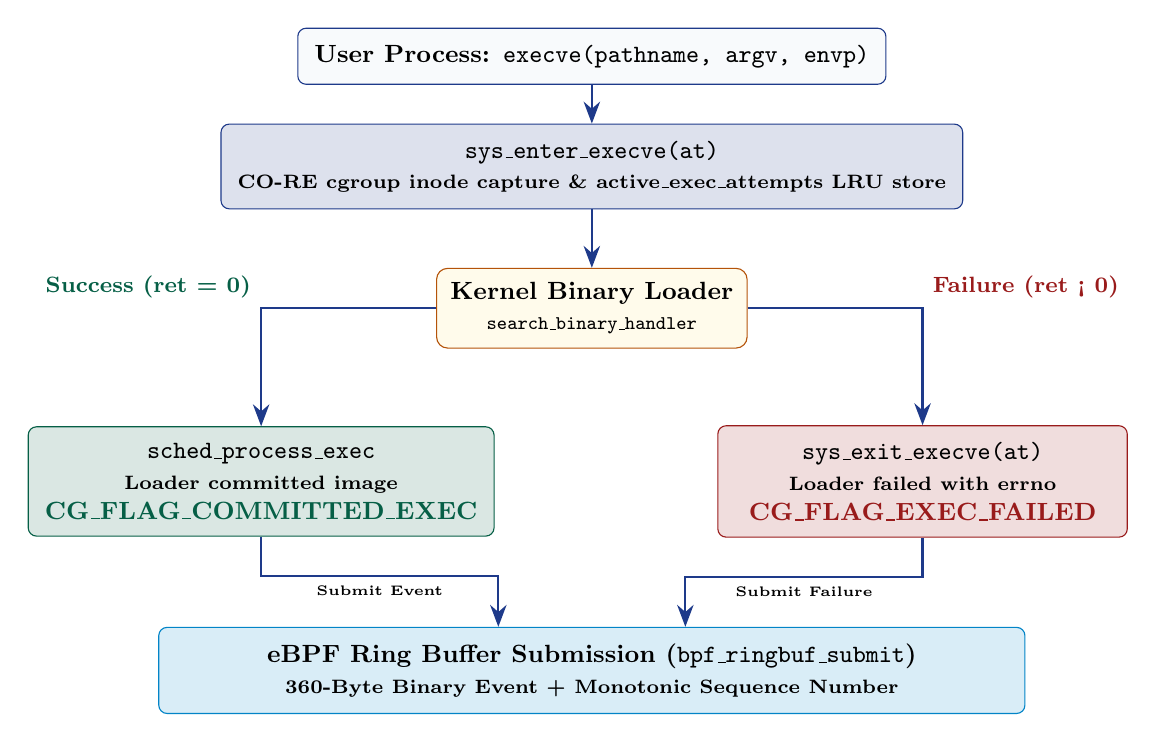
\begin{tikzpicture}[
    box/.style={rectangle, draw=primaryblue, fill=boxbg, rounded corners=3pt, font=\small\bfseries, align=center, inner sep=6pt},
    decision/.style={rectangle, draw=amber, fill=lightamber, rounded corners=4pt, font=\small\bfseries, align=center, inner sep=5pt},
    arrow/.style={-{Stealth[scale=1.2]}, thick, draw=primaryblue}
]
    \node[box, minimum width=6cm] (app) at (0, 6.2) {User Process: \texttt{execve(pathname, argv, envp)}};
    \node[box, fill=primaryblue!15, minimum width=8cm] (enter) at (0, 4.8) {\texttt{sys\_enter\_execve(at)}\\ \scriptsize CO-RE cgroup inode capture \& active\_exec\_attempts LRU store};
    \node[decision] (loader) at (0, 3.0) {Kernel Binary Loader\\ \scriptsize\textnormal{\texttt{search\_binary\_handler}}};

    \node[box, fill=darkgreen!15, draw=darkgreen, minimum width=5.2cm] (sched) at (-4.2, 0.8) {\texttt{sched\_process\_exec}\\ \scriptsize Loader committed image\\ \textbf{\textcolor{darkgreen}{CG\_FLAG\_COMMITTED\_EXEC}}};
    \node[box, fill=crimson!15, draw=crimson, minimum width=5.2cm] (exit) at (4.2, 0.8) {\texttt{sys\_exit\_execve(at)}\\ \scriptsize Loader failed with errno\\ \textbf{\textcolor{crimson}{CG\_FLAG\_EXEC\_FAILED}}};

    \node[box, fill=accentblue!15, draw=accentblue, minimum width=11cm] (rb) at (0, -1.6) {eBPF Ring Buffer Submission (\texttt{bpf\_ringbuf\_submit})\\ \scriptsize 360-Byte Binary Event + Monotonic Sequence Number};

    \draw[arrow] (app) -- (enter);
    \draw[arrow] (enter) -- (loader);
    \draw[arrow] (loader) -| node[above left, font=\footnotesize\bfseries\color{darkgreen}]{Success (ret = 0)} (sched.north);
    \draw[arrow] (loader) -| node[above right, font=\footnotesize\bfseries\color{crimson}]{Failure (ret < 0)} (exit.north);
    \draw[arrow] (sched.south) -- ++(0,-0.5) -| node[pos=0.25, below, font=\tiny\bfseries]{Submit Event} (rb.155);
    \draw[arrow] (exit.south) -- ++(0,-0.5) -| node[pos=0.25, below, font=\tiny\bfseries]{Submit Failure} (rb.25);
\end{tikzpicture}

\end{document}
